% DUDAS
% LAS REFERENCIAS DEBERIAN IR EN LAS REFERENCIAS DEL DOCUMENTO EN GENERAL
% LA CALIDAD DEL DOCUMENTO ES PESIMA
% LOS REQUISITOS DE INFORMACION SON NO FUNCIONALES
% HE REPETIDO DEMASIADAS VECES LO QUE HACE MI SIMULADOR
% EN LA MAYORIA DE LAS SECCIONES HE RELLENADO MAS BIEN POCO
% ME PARECEN POCOS REQUISITOS EN GENERAL, PERO NO SE ME OCURREN MAS

% DUDAS TUTORIA
%no se si poner aqui lo de la pagina web. tipo, que no hay suficientes opciones software para el publico general.


% TODO
% PONER QUE NOS REFERIMOS A SOFTWARE, SISTEMA Y ESO A LO MISMO
\chapter{Especificación de requisitos}

\section{Introducción}

\subsection{Propósito}
%mejorar
El objetivo de esta especificación es definir de manera clara, concisa y precisa las funciones y restricciones que tendrá la aplicación que se desea desarrollar. Al ser un trabajo individual, irá dirigido principalmente a mí, que haré de equipo de desarrollo.

\subsection{Alcance}
%rescribir subsection entera
El proyecto será conocido de ahora en adelante como ``\myTitle''. Por lo tanto, al hacer referencia a ``proyecto'', ``software'', ``simulador'', ``aplicación'' y ``aplicación gráfica'', me referiré a lo mismo.

\bigskip

% repes: carrera
Este sistema se encargará de simular carreras de coches, donde los pilotos tendrán distintas características que variarán dependiendo de las condiciones de la carrera e influirán en su desempeño. El usuario podrá modificar el estado de cada piloto en tiempo real, observando como estos afectan al comportamiento del vehículo.

\bigskip

Además, el software permitirá modificar una serie de ajustes antes de simular la carrera, de acuerdo a las preferencias del usuario. Algunos parámetros son: el número de vehículos, las aptitudes de cada piloto, el tipo de coche y la velocidad máxima. De esta manera, se podrán crear carreras personalizadas de acuerdo a las necesidades del usuario.

\subsection{Definiciones, siglas y abreviaturas}

\begin{itemize}
    \item \textbf{Definiciones: }
        \begin{itemize}
            \item \textbf{Usuario: }Persona que utiliza el sistema con el objetivo de obtener los resultados de la carrera personalizada.
            \item \textbf{Simulación: }Se refiere a la ejecución de una carrera en la aplicación.
            \item \textbf{Piloto: }Conductor de un vehículo en la simulación. Será 
            \item \textbf{Aguante mental y físico: }Condiciones que tiene un piloto durante la carrera y que son modificadas durante la simulación, pudiendo afectar a su conducción.
            \item \textbf{Agresividad: }Factor que afectará al piloto durante la carrera, haciendo que si sube cometa más errores.
            \item \textbf{Experiencia: }Parámetro del piloto que no varía durante la carrera y que indica la habilidad que tiene para tomar decisiones.
        \end{itemize}
    \item \textbf{Siglas: }
    \begin{itemize}
        \item \textbf{FPS: }\textit{Frames Per Second}. Son los fotogramas (imágenes) que muestra el sistema cada segundo. Si son lo suficientemente altos, se genera la ilusión de movimiento.
    \end{itemize}
\end{itemize}

% \subsection{Referencias}

% Los siguientes documentos y enlaces se han consultado para crear este capítulo:

% \begin{itemize}
%     \item Ingeniería del Software. Ejercicio en clase, unidad 3: Requerimientos del Software. LSI (UGR). \url{https://lsi2.ugr.es/~mvega/docis/aluwork/colectivo/Ejercicio%20en%20clase%20version%202}
%     \item fusm calidad del software. \url{https://sites.google.com/site/fusmcalidaddelsoftware/proyecto/g-informe-de-especificacion-de-requerimientos/3-requisitos-especificos/3-5-atributos-del-sistema}
% \end{itemize}

\subsection{Visión general}
% rescribir
Este capítulo constará de tres secciones: %Introducción, descripción global, y requisitos específicos. 

\bigskip

En esta primera sección se muestra la introducción y la visión general de la especificación de requisitos.

\bigskip

En la sección 2 se proporcionará una descripción general del sistema a construir, con el fin de conocer las funciones principales, datos requeridos, restricciones y otros aspectos relevantes. 

\bigskip

En la sección 3 se definen detalladamente los requisitos que debe cumplir el sistema en el momento de su desarrollo.

\section{Descripción general}
\subsection{Perspectiva del producto}

\begin{figure}[H]
    \centering
    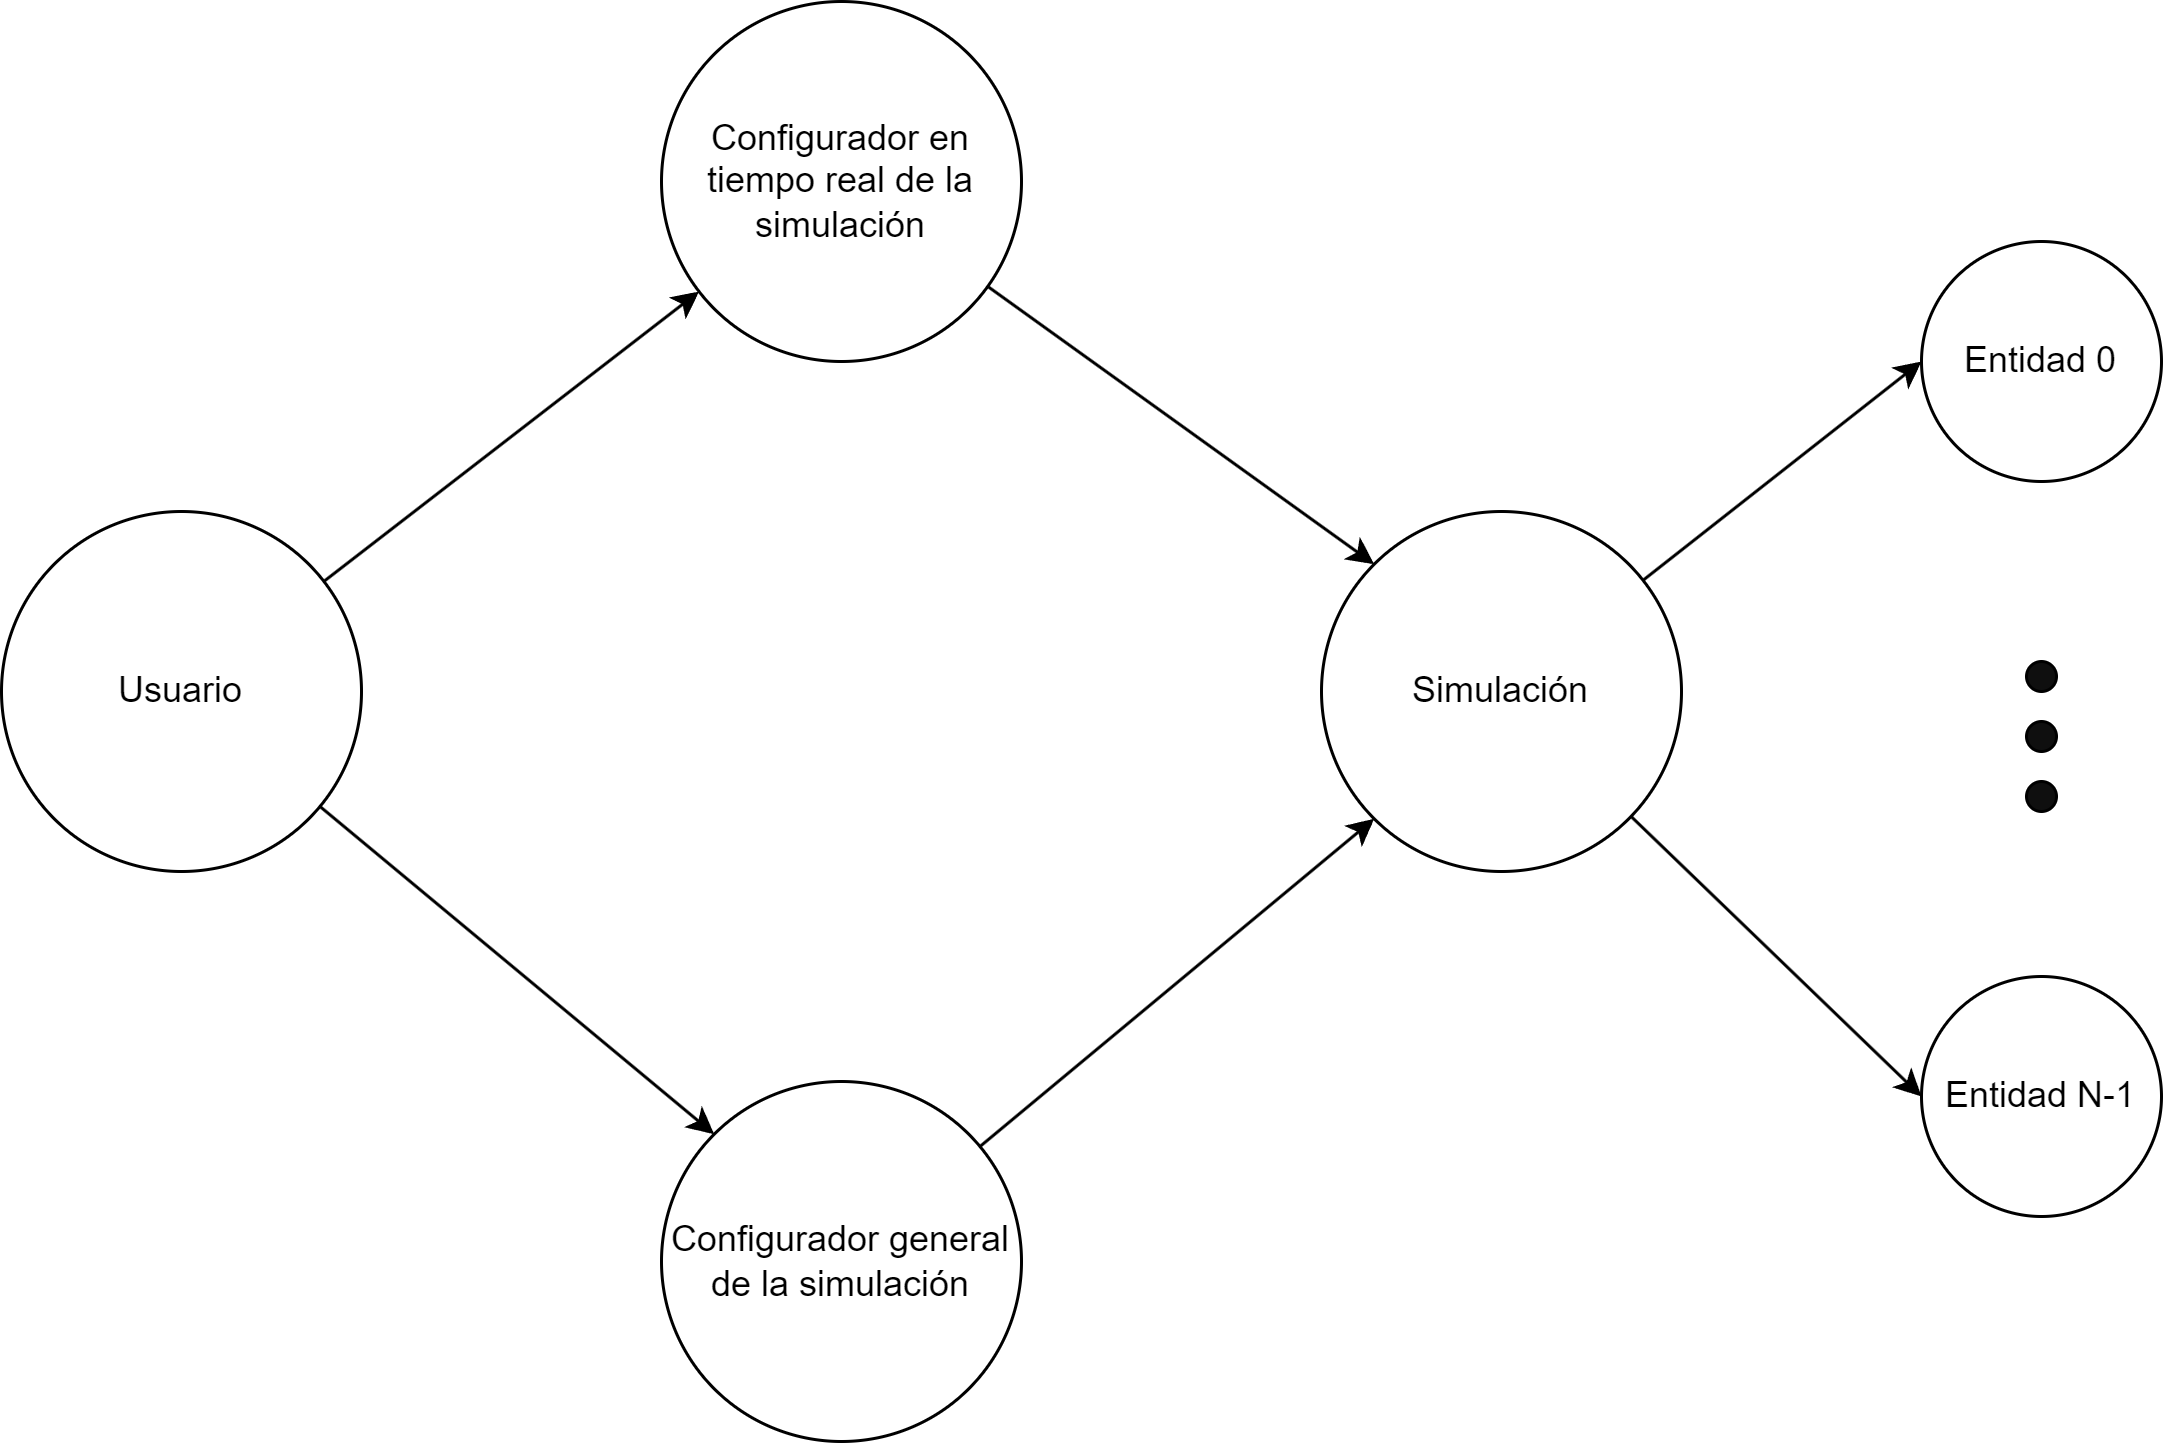
\includegraphics[width=0.8\textwidth]{imagenes/grafo-sistema.drawio.png}
    \caption{Grafo de los distintos componentes del sistema.}
 \end{figure}

El software se diseñará como una aplicación gráfica que permitirá a los usuarios simular carreras de coches, permitiendo configurar parámetros antes de la simulación y durante la carrera. El sistema recopilará información sobre la situación de carrera de cada piloto, y utilizará estos datos para simular el desempeño de cada uno en tiempo real.

\bigskip

Los usuarios interactuarán con el sistema a través de una interfaz gráfica con la que podrán modificar todos los ajustes que estimen convenientes.

\bigskip

Además, será un sistema independiente, al no necesitar interactuar con otros sistemas externos.

\subsection{Funciones del producto}

Las funciones principales de la aplicación son las siguientes:

\begin{itemize}
    \item 
    %Configuración de los parámetros antes de la carrera: 
    % Otorgará la posibilidad de 
    Configurar las distintas opciones antes de la carrera como: número de pilotos, aptitudes de cada uno, tipo de vehículo, velocidad máxima y número de vueltas. 
    
    \item Calcular el estado del piloto según las condiciones actuales de la carrera, de manera que si su estado empeora, cometerá más errores y si mejora, cometerá menos errores, todo en tiempo real.
    
    \item Modificar el estado de los pilotos durante la carrera, con independencia de las condiciones de la misma, pudiendo ver en tiempo real como afecta el cambio producido.
\end{itemize}

Y tendrá otras funciones como:

\begin{itemize}
    \item Pausar la simulación.
    \item Acelerar o reducir la velocidad de simulación.
    \item Cambiar la hora del día.
\end{itemize}

\subsection{Características de los usuarios}

Es recomendable que los usuarios tengan conocimientos básicos de informática, pero no es necesario que sepan como funcionan las carreras, ya que el proceso se encuentra automatizado. 

\subsection{Restricciones}

Las restricciones que tendrá la aplicación son las siguientes:

\begin{itemize}
    \item \textbf{RES1.-} Para el apartado gráfico y la interfaz, se utilizará el motor gráfico \textit{Unreal Engine}.
    \item \textbf{RES2.-} Una vez pausada la simulación, no se podrá modificar su velocidad.
    \item \textbf{RES3.-} El número de pilotos en la carrera no puede ser menor o igual a 1.
    \item \textbf{RES4.-} Las aptitudes de cada piloto antes de la carrera tienen que ser mayores que 0.
    % \item \textbf{RES5.-} La velocidad máxima no podrá ser menor de 150 km/h.
\end{itemize}

\subsection{Suposiciones y dependencias}

% Los requisitos descritos pueden estar sujetos a cambios en función de la evolución del proyecto y la posible adición de nuevas funcionalidades. 

% \bigskip

Este sistema funciona de forma independiente, por lo que no es necesario comunicarse con otros sistemas externos o instalar ningún programa adicional, excepto el propio simulador.

\bigskip

También se asume que el sistema operativo instalado es Windows en sus versiones 10 u 11.

\subsection{Requisitos específicos}

\subsubsection{Requisitos funcionales}

\begin{itemize}
    \item \textbf{RF1.- Modificación de parámetros antes de la carrera:} El sistema debe permitir modificar los parámetros antes de ejecutar la simulación.
    \item \textbf{RF2.- Visualización del estado de los pilotos:} El usuario podrá ver el estado de cada piloto durante la carrera, para poder realizar operaciones sobre el mismo, si lo ve necesario.
    \item \textbf{RF3.- Modificación del estado de los pilotos durante la carrera:} El sistema permitirá modificar el estado de los pilotos en tiempo real.
    \item \textbf{RF4.- Actualización de la velocidad de simulación:} El sistema permitirá actualizar la velocidad entre varias opciones predefinidas.
    \item \textbf{RF5.- Pausado y reanudado de la simulación:} El sistema permitirá pausar y reanudar la simulación que está en curso.
    \item \textbf{RF6.- Características del simulador:} El sistema debe simular la conducción de varios pilotos en una carrera de coches, como adelantamientos y sorteo de obstáculos, entre otros. Los pilotos tendrán un conjunto de condiciones que variarán durante la carrera y que afectarán a su rendimiento.
    \item \textbf{RF7.- Exportación de la configuración de la simulación:} El sistema permitirá almacenar la configuración de la carrera en un fichero para su posterior importación.
    \item \textbf{RF8.- Importación de la configuración de la simulación:} El sistema permitirá importar la configuración de la simulación.
    \item \textbf{RF9.- Visualización de la vuelta actual:} El sistema deberá realizar el cálculo y la visualización de la vuelta actual.
\end{itemize}


\subsubsection{Requisitos de soporte}

\begin{itemize}
    % \item RNF1.- El sistema debe ser ejecutado en un entorno Windows 10 o Windows 11.
    \item \textbf{RNF1.-} El sistema se ejecutará en los sistemas operativos Windows 10 y Windows 11.
\end{itemize}

\subsubsection{Requisitos de usabilidad}

\begin{itemize}
    \item \textbf{RNF2.-} La interfaz deberá ser fácil de usar e intuitiva para los usuarios, de manera que puedan navegar por la misma sin demasiada dificultad.
    \item \textbf{RNF3.-} El tamaño del texto y el estilo de fuente deben ser adecuados para facilitar su lectura.
\end{itemize}

\subsubsection{Requisitos de rendimiento}

\begin{itemize}
    \item \textbf{RNF4.-} El sistema deberá tardar, como máximo, 50 milisegundos (unos 20 FPS) en ejecutar cada paso de la simulación.
    \item \textbf{RNF5.-} El cambio manual del estado de un piloto debe ser reflejado en la simulación en menos de 10 segundos.
\end{itemize}

\subsubsection{Requisitos de información del sistema}

\begin{itemize}
    \item \textbf{RI1.- Datos de los pilotos:} Nombre, nacionalidad, aguante mental y físico, agresividad y experiencia.
    % \begin{itemize}
    %     \item Nombre
    %     \item Nacionalidad
    %     \item Aguante mental
    %     \item Aguante físico
    %     \item Agresividad
    %     \item Experiencia
    % \end{itemize}
    \item \textbf{RI2.- Datos del simulador:} Velocidad de simulación, hora actual, número de vueltas, vuelta actual y número de vehículos.
\end{itemize}

\subsubsection{Aspectos legales}

La simulación no va a guardar ningún tipo de dato privado ni asociable a un individuo, haciendo que todos los datos sean anónimos. Por tanto, no es necesario seguir ningún tipo de tratamiento especial con la información insertada en la aplicación.

\subsubsection{Interfaz de usuario}

La interfaz de usuario que se utilizará para configurar los parámetros previos a la carrera estará compuesta por varios deslizadores para ajustar distintos parámetros de la simulación. Además, habrá otra ventana para modificar algunas características de los pilotos y dos botones para importar y exportar la configuración.

\bigskip

Durante la carrera, la interfaz de usuario tendrá un aspecto similar al de las carreras reales, con un contador de vueltas y la posición de los pilotos a la izquierda. Asimismo, se podrá pulsar sobre un piloto para ver y modificar su estado en tiempo real.

\newpage

Los bocetos de dichas interfaces son las siguientes:
% La estructura que tendrá la interfaz de usuario es la siguiente:

\begin{figure}[H]
    \centering
    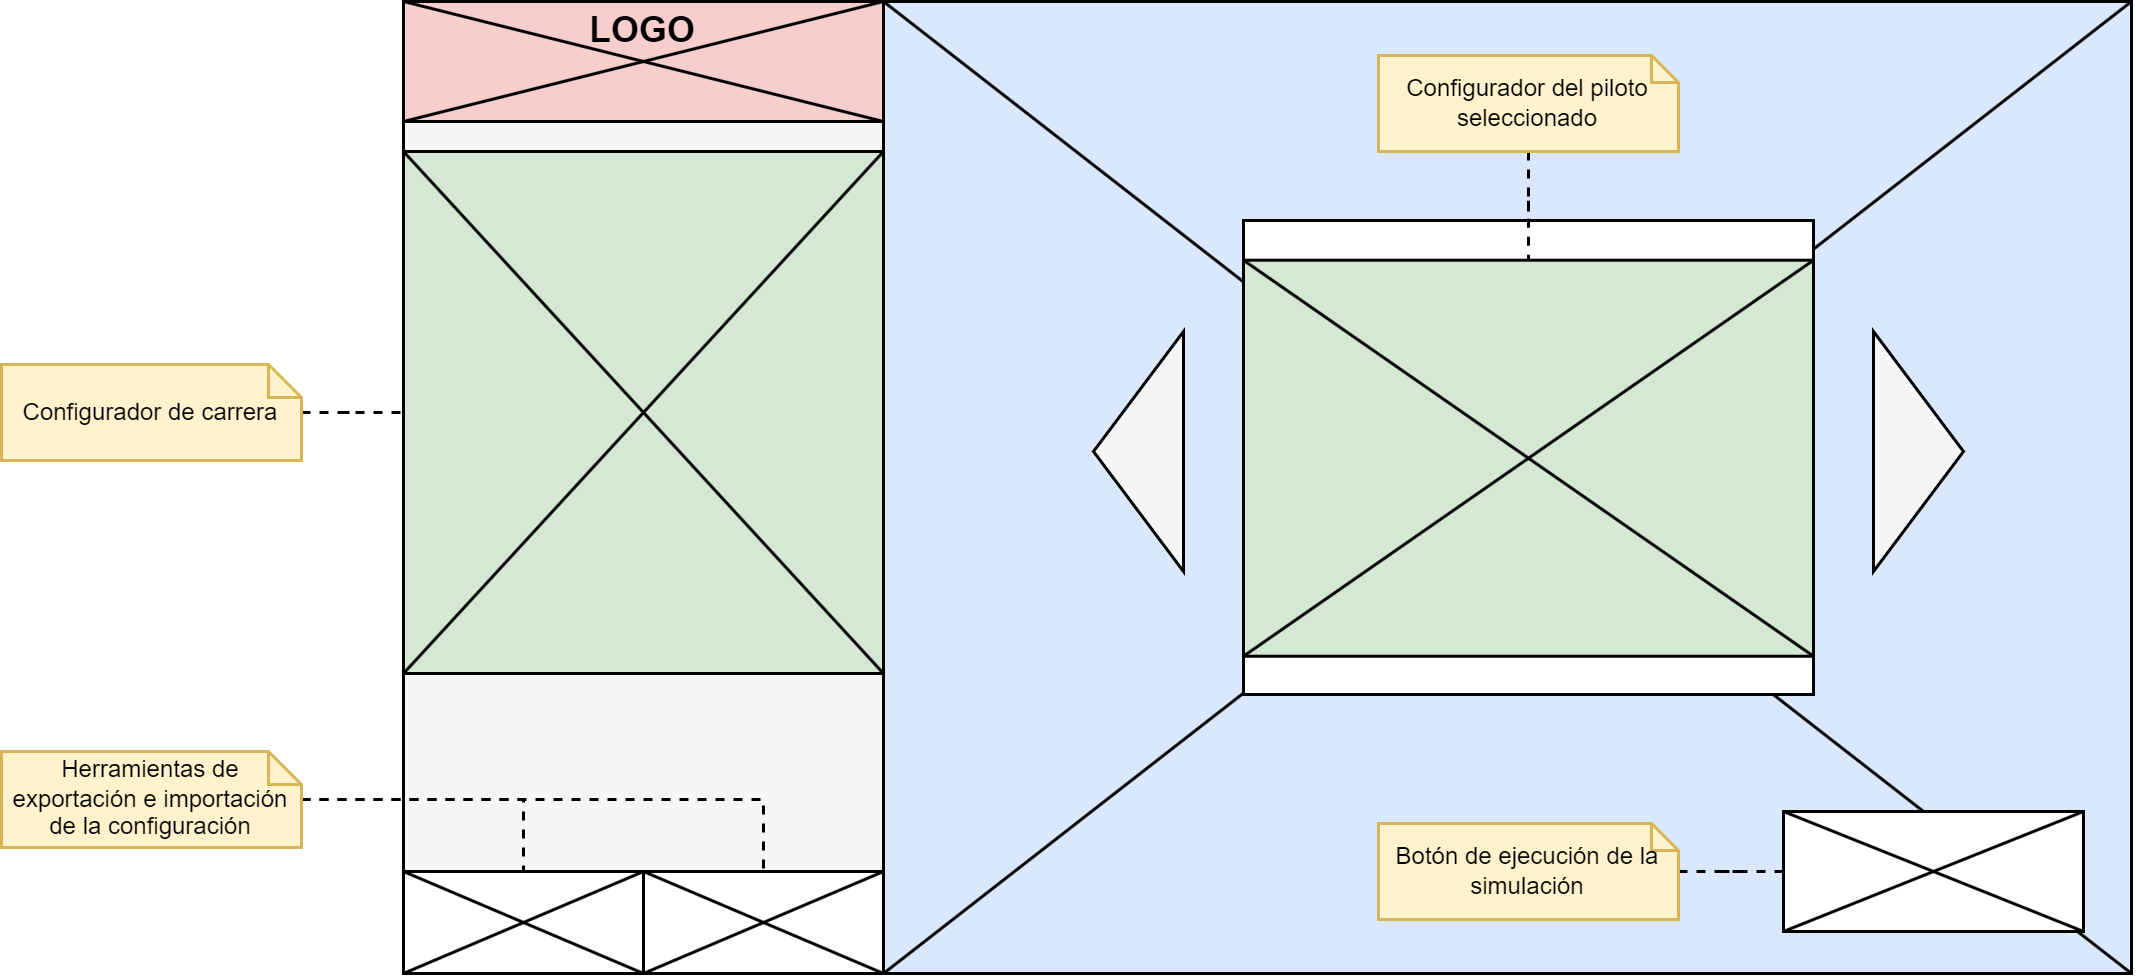
\includegraphics[width=\textwidth]{imagenes/pag1-proto.png}
    \caption{Prototipo del configurador antes de la carrera.}
 \end{figure}

 \begin{figure}[H]
    \centering
    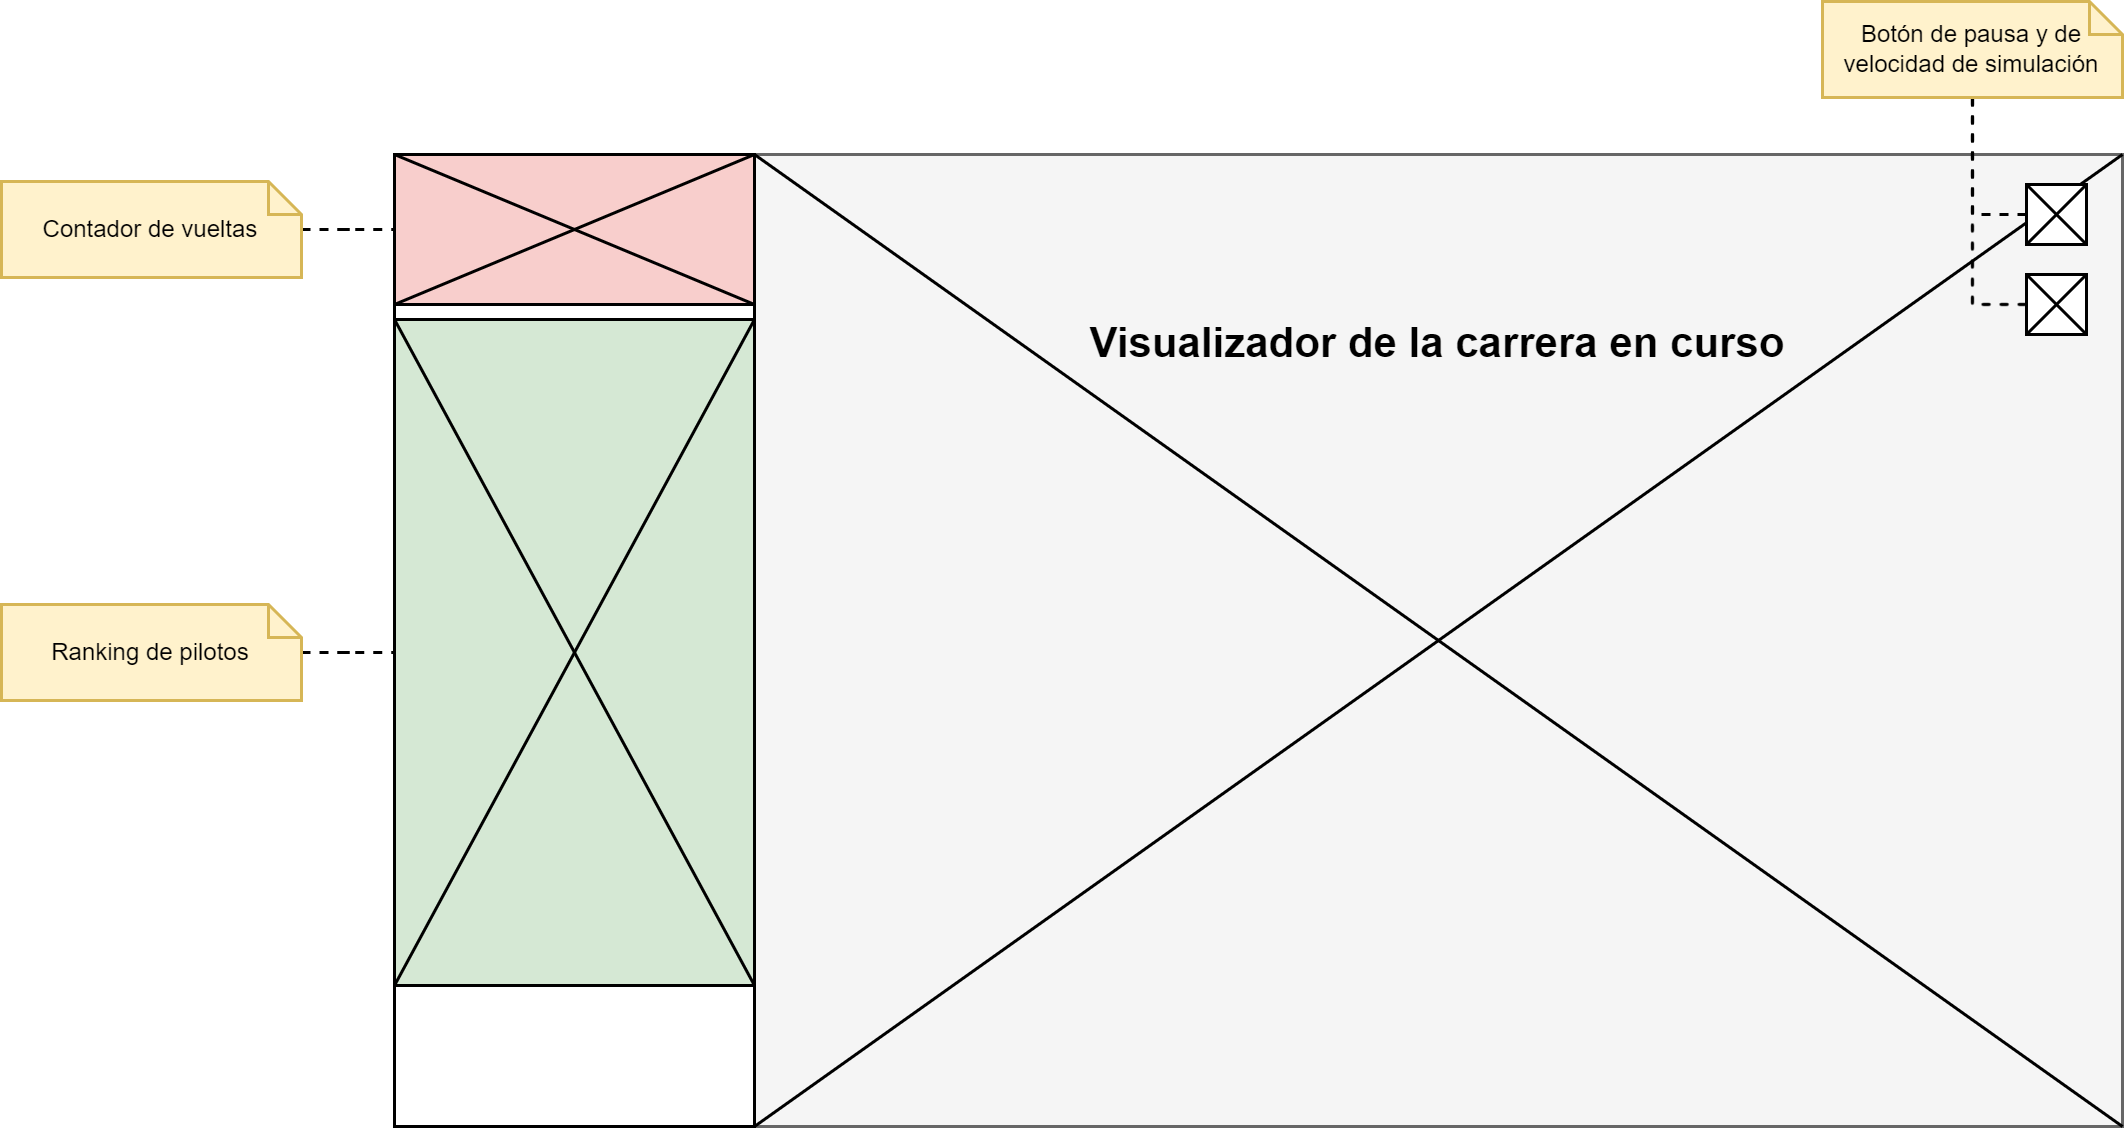
\includegraphics[width=\textwidth]{imagenes/pag2-proto.png}
    \caption{Prototipo de la interfaz de las opciones durante la carrera.}
 \end{figure}